\documentclass{article}
\usepackage{tikz}
\usetikzlibrary{arrows}
\usetikzlibrary{graphs}
\usetikzlibrary{shapes.misc}
\usetikzlibrary{calc}

\begin{document}
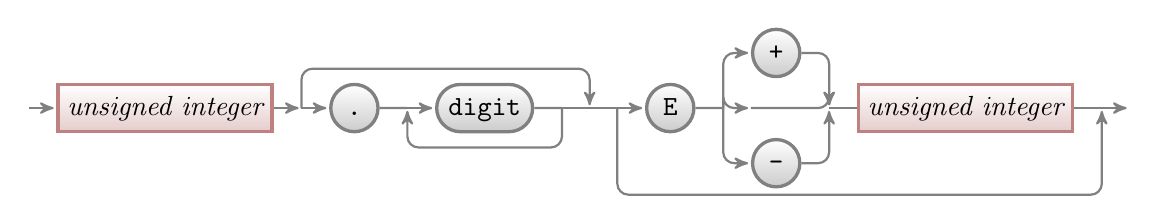
\begin{tikzpicture}[>=stealth', thick, black!50, text=black,
  every new ->/.style={shorten >=1pt},
  graphs/every graph/.style={edges=rounded corners},
  skip loop/.style = {to path={-- ++(0,#1) -| (\tikztotarget)}},
  hv path/.style = {to path={-| (\tikztotarget)}},
  vh path/.style = {to path={|- (\tikztotarget)}},
  node distance=5mm,
  text height=1.5ex,text depth=.25ex,
  terminal/.style={rounded rectangle,minimum size=6mm,very thick,draw=black!50,top color=white,bottom color=black!20,font=\ttfamily},
  nonterminal/.style={rectangle,minimum size=6mm,very thick,draw=red!50!black!50,top color=white,bottom color=red!50!black!20,font=\itshape}]

  \graph[grow right sep, branch down=7mm] {
    /                    [coordinate]  ->
    unsigned integer     [nonterminal] ->
    p1                   [coordinate]  ->
    "."                  [terminal]    --
    p2                   [coordinate]  ->
    digit                [terminal]    --
    p3                   [coordinate]  --
    p4                   [coordinate]  --
    p5                   [coordinate]  ->
    E                    [terminal]    --
    q1                   [coordinate]  -> [vh path]
    { [nodes={yshift=7mm}]
      "+"                [terminal],
      "q2/"              [coordinate],
      "-"                [terminal]
    }                                  -> [hv path]
    q3                   [coordinate]  --
    /unsigned integer    [nonterminal] --
    p6                   [coordinate]  ->
    /                    [coordinate];

   p1 ->[skip loop=5mm]   p4;
   p3 ->[skip loop=-5mm]  p2;
   p5 ->[skip loop=-11mm] p6;
  };
\end{tikzpicture}
\end{document}
